\section{Privacy Via Chameleon}
\label{sec:tech}
The results in the previous section demonstrate the huge utility loss in the perturbed output after adding noise to the extracted representative instance to guarantee privacy. In this section, we propose a novel uncertainty-aware algorithm called Chameleon. Chameleon enables unifying and grained control over the noise injected into the \emph{original uncertain} graph. This qualifies Chameleon to provide enough privacy guarantee in better utility. 

\subsection{The Chameleon framework}
\begin{algorithm}
% {\scriptsize
	\begin{algorithmic}[1]
    	\item[] {\textbf{Input:}~Uncertain graph $\mathcal{G}$, adversary knowledge $\mathcal{K}$, obfuscation level $k$, tolerance level $\epsilon$, size multiplier $c$ and white noise level $q$ }
        \item[] {\textbf{Output:}~The anonymized result $\tilde{\mathcal{G}}_{obf}$}
     	\STATE {$\sigma_{l} \leftarrow 0$; $\sigma_{u} \leftarrow 1$} \\
        \REPEAT
        \STATE{$\langle \tilde{\epsilon}, \tilde{\mathcal{G}} \rangle$ $\leftarrow$ \texttt{GenObf}($\mathcal{G},k,\epsilon,c,q,\sigma_{u}, \mathcal{K}$)} \\
        \STATE{{\bf if} $\tilde{\epsilon}=1$ (fail) {\bf then} $\sigma_{l} \leftarrow \sigma_{u}$; $\sigma_{u} \leftarrow 2\sigma_{u}$}
        \UNTIL{$\tilde{\epsilon} \neq 1 $} \\
        \REPEAT
        	\STATE {$\sigma \leftarrow (\sigma_{u}+\sigma_{l})/2$}
            \STATE {$\langle \tilde{\epsilon}, \tilde{\mathcal{G}} \rangle \leftarrow \texttt{GenObf}(\mathcal{G},k,\epsilon,c,q,\sigma_{u}, \mathcal{K})$}
            \STATE {{\bf if} $\tilde{\epsilon} =1$~{\bf then}~$\sigma_{l} \leftarrow \sigma$}
            \STATE {{\bf else} $\sigma_{u} \leftarrow \sigma;~~\tilde{\mathcal{G}}_{obf} \leftarrow \tilde{\mathcal{G}}$}
        \UNTIL{$\sigma_{u}-\sigma_{l}$ is enough small}
        % \COMMENT{\textcolor{blue}{\scriptsize Binary search for better obfuscation}}
        \STATE {return $\tilde{\mathcal{G}}_{obf}$}
    	\caption{\SysName Iterative Skeleton}
	 \label{alg:Skeleton}
    \end{algorithmic}
    % }
\end{algorithm}
\vspace{-5pt}

\textbf{Contribution.}~~The conventional schemes are plausible if the operating edge probability is binary, which is unreasonable when dealing with uncertain graphs. Our goal is to develop a anonymization mechanism that reduced the amount of noise that must be added to achieve a given privacy level for \emph{uncertain} graphs. Our insight is to shift an existing framework by integrating uncertainty semantics into its core steps.

We now introduce the state-of-art perturbation algorithm~\cite{Boldi_Injecting_2012} that computes the noise needed to injected into the input \emph{determinitic} graph to obtain the desired privacy level. Each selected edge is altered based on a stochastic variable drawn from a trunated normal distribution, $R(\sigma)$. This distribution has density function proportional to the normal distribution, with mean $0$ and variance $\sigma^2$. Thus, small values of $\sigma$ contribute towards better utility, but at the same time they provide lower level of obfuscation. Targeting for high utility, the algorithm aims at injecting the minmal amount of noise need to achieve the required obfuscation. Its computation is achieved via a binary search on the value of the noise parameter $\sigma$, as shown in Algorithm~\ref{alg:Skeleton}. 

The binary search flow is determined by the \texttt{GenObf} function. 
The function \texttt{GenObf} aims at finding a {\keobf} using a given noise parameter $\sigma$.
It returns a pair $\langle \tilde{\epsilon}, \tilde{\mathcal{G}} \rangle$, where $\tilde{\epsilon} =1$ or $\tilde{\epsilon} \le \epsilon$. In the first case, all the attempts fail. In the latter cases, $\tilde{\mathcal{G}}$ is a {\keobf}. 
The function \texttt{GenObf} finds obfuscation candidate in a randomized way, $t$ attempts are performed. Each attempt performs following core steps:
\begin{itemize}
    \item{Select a subset of edges subjects to further alteration;}
    \item{Alter selected edges as the computed amount of noise;}
    \item{Check the solution with/out enough privacy guarantee;}
\end{itemize}
In the following sections, we introduce how to integrate \emph{uncertainty} in edge selection \& alteration. 


\subsection{Uncertainty-aware Edge Selection}
The first challenge is to find out the optimal subset of edges that balances privacy gain and utility loss for further alteration. 
It is a typical combinational optimization problem which involves the consideration over the exponential number of edge combinations. Let alone the infinite possibilities of probability values on the selected edges, which further complicates the problem.

To alleviate combinational intractability, heuristics have been proposed in the context of deterministic graphs. 
They can be classified into two main categories: 
(1)~{\em Anonymity-oriented} heuristics that suggest calibrating the applied noise according to the ``uniqueness". To ``blend" unique nodes into crowds, a larger amount of noise is necessary. ~\cite{Boldi_Injecting_2012,Liu_Towards_2008, Thompson_The_2009,Zhou_Preserving_2008}, and 
(2)~{\em Utility-oriented} heuristics that suggest calibrating the applied noise according to the ``relevance". To preserve graph structure, avoiding large perturbation over ``important" edges~\cite{casasprivacy,Ying_Randomizing_2008,Liu_Privacy_2009,Ninggal_Utility_2015}.
Note that, these two types are complementary to each other. Their combination would introduce a cumulative benefit, which has been confirmed in the deterministic graph anonymization practice~\cite{casasprivacy}. 

\textbf{Contribution.}~~Nevertheless, these two types of heuristics and their combination have not been explored yet in the context of \emph{uncertain} graphs.
In this work, we first extend the idea of \emph{uniqueness} score via a density estimation method. Second, we propose a novel edge relevance that extends well-known graph concepts, such as ``cut edge" for estimating structural errors incurred by edge probability alterations. We design a sampling-based algorithm to compute edge relevance in \emph{uncertain} graphs. Finally, we show how to utilize these \emph{uncertainty}-embedded meta-heuristics to effectively select edges for further alteration. 

\subsection{Uniqueness Score}
Intutively, larger amount of noise should be added at nodes that are less anonymized (i.e, more distinctive) in the original graphs. Thus, we are left asking the question, how to measure the typical level of a given node among the nodes of the original \emph{uncertain} graph. \emph{Uniqueness score} is shown to be an effective metric in the context of deterministic graphs~\cite{Boldi_Injecting_2012}. The formal defintion of uniqueness score is given as follows. 
\begin{definition}
    \textbf{Uniqueness Score~\cite{Boldi_Injecting_2012}}
     Let $P:V \rightarrow  \Omega_{P}$ be a property on the set of nodes $V$ of the graph $\mathcal{G}$, let $d$ be a distance function on $\Omega_{P}$, and let $\theta >0$  be a parameter. 
  Then the $\theta-commonness$ of the property values $\omega \in \Omega_{P}$ is $C_{\theta}(\omega):= \sum_{u \in V} \Phi_{0,\theta}(d(\omega, P(v)))$,   
while the $\theta$-uniqueness of $\omega \in \Omega_{P}$ is $U_{\theta}:= \frac{1}{C_{\theta}(\omega)}$. 
\end{definition} 

Note that, it adopts a parametric way to estimate the probability density function of the property value $\omega$ (i.e., how typical the value is among all the nodes). It place a smooth kernel function $Phi$ with standard variance $\theta$, where $\theta$ implies the spread out of the property value over the domain.
In the previous work~\cite{Boldi_Injecting_2012}, they set $\theta=\sigma$, where $\sigma$ is the standard deviation of the noise generation Gaussian distribution since the larger injected amount of uncertainties indicates that the property values may be spread out in a larger domain. 

In this work, we set $\theta$ equals $\sigma_{\mathcal{G}}$ as the latter represents the spread of property value in the \emph{uncertain graph}. For a given node with the property $\omega$, we can compute its ``uniqueness" score as the reverse of its density. The higher the uniqueness score the less-protected the node and the more anonymization it eventually needs.

\subsection{Reliability Relevance}

\textbf{\emph{Observation}}~~ 
When an uncertain edge is altered (partial added or deleted), it will result in the change of reliability. 
The same amount of alteration performed over different edges may incur significantly different structure change. 
Referring to the example in Figure~\ref{fig:edgeRRGraph}, two vertices $\tt{a}$ and $\tt{e}$ will be assigned the same {\em uniqueness score} due to the exact probabilities associated with their edges. 
As a result, the {\em anonymity-oriented} strategy would select and perturb either of the two edges $(\tt{a},\tt{c})$ and $(\tt{c},\tt{e})$ with the same probability. 
However, the modifications to $(\tt{c},\tt{e})$---which is the only link between two~\emph{reliable} clusters---clearly incurs much larger structure distortion than that on $(\tt{a},\tt{c})$. 
Therefore, edge perturbation needs to consider the structural impact of \emph{uncertain} graph edge alteration.



To this end, we propose a theoretically sound estimation for the {\em ``reliability deviation''} caused by individual uncertain edge modifications in a fine-grained way. 
Following this path, we introduce a new measure, called {\em Edge Reliability Relevance $(\mathcal{E}RR)$}, at the edge level, and an aggregated measure, called {\em Vertex Reliability Relevance $(\mathcal{V}RR)$}, at the vertex level as will be formally defined next. These measures will enable ranking the edges to be targeted for obfuscation in a meaningful utility-based perspective. Besides, we provide an algorithm for computing them efficiently. 


\begin{definition}
    \textbf{Two-terminal Reliability Relevance}
    Given an uncertain graph $\mathcal{G}$, and two nodes $u$ and $v$, 
    the  reliability $R_{u,v}(\mathcal{G})$ as defined in Def.~\ref{d:reliability} is considered as a multivariate function involving all the edge probabilities in $\mathcal{G}$.   
    Thus, given an uncertain edge $e \in \mathcal{G}$, the partial derivative of $R_{u,v}(\mathcal{G})$ w.r.t $e$'s probability 
    variable $p(e)$, denoted as $\mathcal{E}RR^{e}_{u,v}(\mathcal{G})$, represents the sensitivity of the 
    two-terminal reliability $R_{u,v}$ w.r.t $p(e)$ while all others are held constant. 
     It is defined as:  
\begin{equation*}
	\vspace{-0.5em}
    \mathcal{E}RR^{e}_{u,v}(\mathcal{G}) = \frac{\partial R_{u,v}(\mathcal{G})}{\partial \mathit{p}(e)}
    \vspace{-0.5em}
\end{equation*}
\end{definition}


\begin{figure}
  \vspace{-1em}
    %\captionsetup{justification=centering,margin=0cm}
  \subfigure[An uncertain graph]{\label{fig:edgeRRGraph}  %(22)
    \begin{minipage}[l]{0.4\columnwidth}
      \centering
      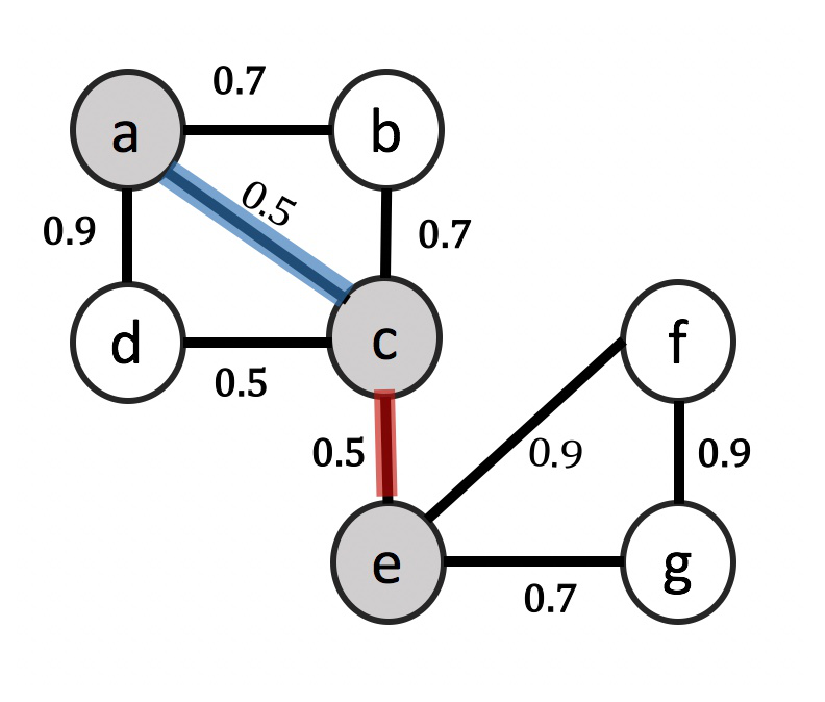
\includegraphics[height=3cm]{ill/edgeSelection.eps}
    \end{minipage}
  }
  \subfigure[The reliability $R_{a,e}$ v.s $p(e)$]{\label{fig:edgeRR}  %(22)
    \begin{minipage}[l]{0.5\columnwidth}
      \centering
      \includegraphics[height=3cm]{ill/rrIll.eps}
    \end{minipage}
  }
    \vspace{-1em}
    \caption{(a) Different edges have different effect on the overall graph reliability. (b) Formal {\em Reliability Relevance } measure. A bigger edge's slope indicates  
     big distortion in reliability under small changes to the edge's probability.}
    \vspace{-0.5em}
\end{figure}


\begin{lemma}
    \textbf{Factorization Lemma}
       Given an uncertain graph $\mathcal{G}$, the reliability of the node pair $(u,v)$, i.e., $R_{u,v}(\mathcal{G})$, can be factorized via a specific uncertain edge $e$ as follows:
    \begin{equation*}
        R_{u,v}(\mathcal{G}) = p(e) R_{u,v} (\mathcal{G}_{e}) + (1-p(e)) R_{u,v} (\mathcal{G}_{\bar{e}} ) 
        \label{eq:fac}
    \end{equation*}
    where uncertain graphs $\mathcal{G}_{e}$ and  $\mathcal{G}_{\bar{e}}$ are identical to the original graph $\mathcal{G}$ with the 
    exception that $e$ is certainly present in the former and certainly not present in the later. 
\end{lemma}


According to the factorization lemma, the partial derivative $\mathcal{E}RR^{e}_{u,v}$ can be rewritten as: 
\begin{equation*}
    \mathcal{E}RR^{e}_{u,v}(\mathcal{G}) = R_{u,v}(\mathcal{G}_{e})-R_{u,v}(\mathcal{G}_{\bar{e}})
\end{equation*}

On one hand, this factorization indicates that for a given edge $e$,  the incurred reliability discrepancy is {\bf linear} to the amount of edge probability difference. 
On the other hand, it indicates that edges with different topological locations have different reliability sensitivity. 
The other crucial point to highlight is that $R_{u,v}(\mathcal{G}_{e}) - R_{u,v} (\mathcal{G}_{\bar{e}}) \ge 0$ is always true since 
all connected pairs in $\mathcal{G}_{e}$ are guaranteed to be a superset or at least equal to that in $\mathcal{G}_{\bar{e}}$.

Considering a single uncertain edge $e$, the derivatives $\mathcal{E}RR^e_{u,v}(\mathcal{G})$ over all 
vertex pairs in $\mathcal{G}$ can be arranged in a $|V|\times |V|$ matrix, and as highlighted above, 
all entires of this matrix equal to or greater than zero.  
By aggregating these derivatives, we can estimate the overall {\em reliability relevance} of edge $e$, denoted as
$\mathcal{E}RR^{e}(\mathcal{G})$, as the sum of all the $\mathcal{E}RR^{e}_{u,v}$ values. That is:
%In this work, we define $RR(e)$ to be reliability relevance of an edge $e$ which can be quantified by the sum of all the $RR_{u,v}(e)$, as  
\begin{align*}
    \mathcal{E}RR^e(\mathcal{G}) &= \sum_{u,v} |\mathcal{E}RR^e_{u,v}(\mathcal{G})| \\
          &= \sum_{u,v} |R_{u,v}(\mathcal{G}_{e}) -R_{u,v}(\mathcal{G}_{\bar{e}})| \\  
         &= \sum_{u,v} R_{u,v} (\mathcal{G}_{e}) - \sum_{u,v} R_{u,v}(\mathcal{G}_{\bar{e}}) 
\end{align*}

Note that $\mathcal{E}RR^e$ equals to the difference of the expected number of 
connected pairs between the two uncertain graphs $\mathcal{G}_{e}$ and $\mathcal{G}_{\bar{e}}$
 by explicit incorporation of edge uncertainty.  
 In the context of edge relevance, reliability relevance can be seen as generalization of cut-edges, 
 which quantifies the impact of partial edge deletion or addition on the connectivity in the uncertain graph. 
The higher reliability relevance score of an edge, the bigger impact of edge perturbation over the overall graph.  

On the basis of these edge-level reliablity relevance, we can now compute a vertex-level reliability relevance of a given vertex (Say $u$) as a weighted sum of reliability relevance of $u$'s edges $\mathtt{E}^{u}$.  
% Fix $u \in \mathcal{G}$ and let $\mathtt{E}^{u}$ be the pairs of vertices that include $v$, we have 
\begin{equation*}
    \vspace{-0.5em}
    \mathcal{V}RR^{u}(\mathcal{G})=\sum_{e \in \mathtt{E}^{u}} p(e)  \mathcal{E}RR^{e}(\mathcal{G})
    \vspace{0.5em}
\end{equation*}

The $\mathcal{V}RR^{u}(\mathcal{G})$  is a measure of the expected impact of vertex modification on the graph reliability. Namely, the higher the vertex's reliability relevance, the larger reliability distortion introduced by modification associated with its edges.

\textbf{Reliability Relevance Evaluation}
Given this theoretical foundation, the challenge is how to evaluate the reliability relevance of edges in  a given uncertain graph efficiently ($\mathcal{E}RR-$eval). 
For each edge $e$, we need to measure the reliability difference over $\mathcal{G}_{e}$ and $\mathcal{G}_{\bar{e}}$. 
This evaluation involves the two-terminal reliability detection problem, which is known to be NP-complete~\cite{MOBall}.   


A baseline algorithm for $\mathcal{E}RR-$eval is to use the
Monte Carlo sampling. More precisely, we sample $N$ possible
worlds of the input uncertain graph, where $N$ is large enough (around $1,000$) to guarantee high approximation accuracy. 
Over each sampled possible world (Say $G$), we carry out a connected-component computation algorithm to count 
the number of connected pairs $cc(G)$. Then, the count on the original uncertain graph $cc(\mathcal{G})$ can be estimated by taking the average over the sampled deterministic graphs. 

\begin{theorem}
	The complexity of the baseline $\mathcal{E}RR-$eval algorithm is $\mathcal{O} (|E| \cdot  N \alpha(|V|) |E| )$ where $\alpha$ is the inverse Ackermann function.  
\end{theorem}

{\bf Proof sketch} The time complexity of the connected component detection algorithm based on the union-find method is $\mathcal{O}(\alpha(|V|) |E|)$~\cite{Wredman:1989:CPC:73007.73040}. Consequently, computing the $\mathcal{E}RR$ for an edge over the $N$ possible worlds takes time $\mathcal{O}(N \alpha(|V|) |E|)$, and the total time complexity for all the edges is $\mathcal{O} (|E| \cdot  N \alpha(|V|) |E|)$. 


\begin{figure}
	\centering
    \includegraphics[width=1\linewidth]{ill/rrEval.pdf}
    \vspace{-1em}
    \caption{\small Reused sampling estimator for $\mathcal{E}RR$ }
    \label{fig:rrEval}
%     \vspace{-1em}
\end{figure}
Obviously, the baseline algorithm is inefficient when the input uncertain graph is very large (it is quadratic in the number of edges). Here, we present a efficient algorithm for $\mathcal{E}RR$ evaluation in Algorithm~\ref{alg:RReval}. Its basic idea is to re-use the connected components detection result of samples as illustrated in~\ref{fig:rrEval}. For each edge $e$, we group the sampled possible worlds according to the edge existence (Line 4-6), then get the sampled average of $cc$ for each group as accurate approximation of $cc(\mathcal{G}_{e})$ and $cc(\mathcal{G}_{\bar{e}})$. By this way, we bring the the evaluation of edge reliability relevance to the realm.  

\begin{theorem}
	The time complexity of Algorithm\ref{alg:RReval} $\mathcal{E}RR-$val is $\mathcal{O}(N \alpha(|V|) |E|)$ where $N$ is the number of samples.
\end{theorem}



\begin{algorithm}[!tb]
{\scriptsize
    \begin{algorithmic}[1]
       \item[] {\textbf{Input:} ~$\mathcal{G}=(V,E,\mathit{p})$, $N$ is the number of sampled graphs;~}
       \item[] {\textbf{Output:} ~$\mathcal{E}RR$ Reliability relevance of edges in $\mathcal{G}$}
    \STATE {$CC_{e} \leftarrow  \mathbf{0} $, $CC_{\bar{e}} \leftarrow \mathbf{0}$}
    \FOR{i=1 \TO N }
    \STATE {$G \leftarrow $  A deterministic sampled instance}
    \STATE {$Ind(G)$ is edge existence of sampled graph $\mathcal{G}$}
    \STATE {$cc(G) \leftarrow $ the number of connected pairs of $G$}
    \STATE {$CC_{e}+=Ind(G) \cdot cc(G)$,$CC_{\bar{e}}+=(\mathbf{1}-Ind(G)) \cdot cc(G)$ }
    \ENDFOR
    \STATE{$\mathcal{E}RR= CC_{e}/\mathit{p} - CC_{\bar{e}}/{\mathbf{1}-\mathit{p}}$}
         \caption{Edge Reliability Relevance Evaluation}
        \label{alg:RReval}
    \end{algorithmic}
    }
\end{algorithm}

\textbf{Reliability Relevance Evaluation}
Given this theoretical foundation, the challenge is how to evaluate the reliability relevance of edges in  a given uncertain graph efficiently ($\mathcal{E}RR-$eval). 
For each edge $e$, we need to measure the reliability difference over $\mathcal{G}_{e}$ and $\mathcal{G}_{\bar{e}}$. 
This evaluation involves the two-terminal reliability detection problem, which is known to be NP-complete~\cite{MOBall}.   


A baseline algorithm for $\mathcal{E}RR-$eval is to use the
Monte Carlo sampling. More precisely, we sample $N$ possible
worlds of the input uncertain graph, where $N$ is large enough (around $1,000$) to guarantee high approximation accuracy. 
Over each sampled possible world (Say $G$), we carry out a connected-component computation algorithm to count 
the number of connected pairs $cc(G)$. Then, the count on the original uncertain graph $cc(\mathcal{G})$ can be estimated by taking the average over the sampled deterministic graphs. 

\begin{theorem}
	The complexity of the baseline $\mathcal{E}RR-$eval algorithm is $\mathcal{O} (|E| \cdot  N \alpha(|V|) |E| )$ where $\alpha$ is the inverse Ackermann function.  
\end{theorem}

{\bf Proof sketch} The time complexity of the connected component detection algorithm based on the union-find method is $\mathcal{O}(\alpha(|V|) |E|)$~\cite{Wredman:1989:CPC:73007.73040}. Consequently, computing the $\mathcal{E}RR$ for an edge over the $N$ possible worlds takes time $\mathcal{O}(N \alpha(|V|) |E|)$, and the total time complexity for all the edges is $\mathcal{O} (|E| \cdot  N \alpha(|V|) |E|)$. 


\begin{figure}
	\centering
    \includegraphics[width=1\linewidth]{ill/rrEval.pdf}
    \vspace{-1em}
    \caption{\small Reused sampling estimator for $\mathcal{E}RR$ }
    \label{fig:rrEval}
%     \vspace{-1em}
\end{figure}
Obviously, the baseline algorithm is inefficient when the input uncertain graph is very large (it is quadratic in the number of edges). Here, we present a efficient algorithm for $\mathcal{E}RR$ evaluation in Algorithm~\ref{alg:RReval}. Its basic idea is to re-use the connected components detection result of samples as illustrated in~\ref{fig:rrEval}. For each edge $e$, we group the sampled possible worlds according to the edge existence (Line 4-6), then get the sampled average of $cc$ for each group as accurate approximation of $cc(\mathcal{G}_{e})$ and $cc(\mathcal{G}_{\bar{e}})$. By this way, we bring the the evaluation of edge reliability relevance to the realm.  

\begin{theorem}
	The time complexity of Algorithm\ref{alg:RReval} $\mathcal{E}RR-$val is $\mathcal{O}(N \alpha(|V|) |E|)$ where $N$ is the number of samples.
\end{theorem}



\begin{algorithm}[!tb]
{\scriptsize
    \begin{algorithmic}[1]
       \item[] {\textbf{Input:} ~$\mathcal{G}=(V,E,\mathit{p})$, $N$ is the number of sampled graphs;~}
       \item[] {\textbf{Output:} ~$\mathcal{E}RR$ Reliability relevance of edges in $\mathcal{G}$}
    \STATE {$CC_{e} \leftarrow  \mathbf{0} $, $CC_{\bar{e}} \leftarrow \mathbf{0}$}
    \FOR{i=1 \TO N }
    \STATE {$G \leftarrow $  A deterministic sampled instance}
    \STATE {$Ind(G)$ is edge existence of sampled graph $\mathcal{G}$}
    \STATE {$cc(G) \leftarrow $ the number of connected pairs of $G$}
    \STATE {$CC_{e}+=Ind(G) \cdot cc(G)$,$CC_{\bar{e}}+=(\mathbf{1}-Ind(G)) \cdot cc(G)$ }
    \ENDFOR
    \STATE{$\mathcal{E}RR= CC_{e}/\mathit{p} - CC_{\bar{e}}/{\mathbf{1}-\mathit{p}}$}
         \caption{Edge Reliability Relevance Evaluation}
        \label{alg:RReval}
    \end{algorithmic}
    }
\end{algorithm}

\subsection{The \texttt{GenObf} Function}

Now, we are ready to present the details of the  \texttt{GenObf()} function for finding 
a $(k,\epsilon)$-obf instance for an input uncertain graph $\mathcal{G}$ in Algorithm \ref{alg:genObf}. The function receives the parameters that are originally passed to \SysName skeleton (Algorithm~\ref{alg:Skeleton}) including noise parameter $\sigma$.  



\textbf{Uniquness \& Relevance Computation.}~~First, the function start with the computation of the uniqueness score and reliability relevance. (Lines 1 \& 2).
These two invariants correspond to our goals of preserving privacy \& utility.   
Based on these weighting factors, the \texttt{GenObf} then heuristically performs edge selection \& perturbation, i.e, use the noise budget in the most effective way. 


\textbf{Exclusion.}~~Since it is allowed not to obfuscate $\epsilon|V|$ of the nodes per the problem definition, the algorithm leverages the two invariants highlighted above and selects a set $H$ of $\frac{\epsilon}{2}|V|$ nodes with the largest combined uniqueness and reliability relevance scores, and excludes them from subsequent obfuscation efforts. 

\begin{algorithm}[!htb]
% {\scriptsize
	\begin{algorithmic}[1]
    	\item[] {\textbf{Input:}~Uncertain graph $\mathcal{G}=(V,E,\mathit{p})$, $\mathcal{K},k,\epsilon,c,q$, \\and standard deviation $\sigma$ }
        \item[] {\textbf{Output:}~A pair $\langle \tilde{\epsilon}, \tilde{\mathcal{G}} \rangle$} where $\tilde{\mathcal{G}}$ is a $(k,\epsilon)-$obfuscation, or $\tilde{\epsilon}=1$ if fail to find a $\keobf$. 
        \STATE  {\textbf{compute} the uniqueness $U^{v}$ for $v \in V$}
        \STATE  {\textbf{compute} the reliability relevance $\mathcal{V}RR^{v}$ for $v \in V$}
        \STATE  {$Q^{v} \leftarrow U^{v} \cdot \mathcal{V}RR^{v}$ for $v \in V$}
        \STATE  {$H \leftarrow$  the set of $\lceil \frac{\epsilon}{2} |V| \rceil$ with largest $Q^{v}$}
     	\STATE  {Normalized $\mathcal{V}RR^{v}$ for $v \in V \setminus H$}
        \STATE  {$Q^{v} \leftarrow U^{v} \cdot 1-\mathcal{V}RR^{v}$ for $v \in V \setminus H$}
        \STATE {$\tilde{\epsilon} \leftarrow 1$}
   		\FOR{$t$ times} 
%         	\COMMENT{\textcolor{blue} {\scriptsize $\nabla$~~Find an initial successful obfuscation}}
         	\REPEAT  
                \STATE {$E_{C} \leftarrow E$} 
            	\STATE{randomly pick a vertex $u \in V \setminus H$ according to $Q$}
            	\STATE{randomly pick a vertex $v \in V \setminus H$ according to $Q$}
            	% \STATE{draw $w$ uniformly at random from $[0,1]$} 
                % \IF {$(u,v) \in E$} 
                %     \STATE {$E_{C} \leftarrow E_{c} \setminus \lbrace(u,v)\rbrace$ with the probability $p(e)$}
                % \ELSE 
                %     \STATE{$E_{c} \leftarrow E_{c} \cup \lbrace(u,v)\rbrace$}
                % \ENDIF 
                \STATE{{\bf if} $(u,v) \in E$}
                \STATE{{\bf then} $E_{C} \leftarrow E_{c} \setminus \lbrace(u,v)\rbrace$ with the probability $p(e)$}
                \STATE{{\bf else}~$E_{c} \leftarrow E_{c} \cup \lbrace(u,v)\rbrace$} 
            \UNTIL{$E_{C}=c|E|$}
            \FORALL {$e \in E_{C}$} 
            	\STATE {\textbf{compute} $\sigma(e)$}
                \STATE {draw $w$ uniformly at random from $[0,1]$}
                \STATE {{\bf if} $w <q$~{\bf then} $r_{e} \leftarrow U(0,1)$ }
                \STATE {{\bf else} $r_{e} \leftarrow R_{\sigma(e)}$}
				% \IF {$w < q$} \STATE{$r_{e} \leftarrow U(0,1)$}
    %             \ELSE 
    %             \STATE{$r_{e} \leftarrow R_{\sigma(e)}$}
    %             \ENDIF
                \STATE \textbf{$\hat{p}(e) \leftarrow p(e)+ (1-2p(e))\cdot r_{e}$}
            \ENDFOR
            \STATE {$\hat{\epsilon} \leftarrow \text{anonymityCheck}(\tilde{\mathcal{G}})$} 
            % \IF{$\hat{\epsilon}<\epsilon$ and $\hat{\epsilon}< \tilde{\epsilon}$} 
            % \STATE{$\tilde{\epsilon} \leftarrow \hat{\epsilon}$; $\tilde{\mathcal{G}} \leftarrow \hat{\mathcal{G}}$}
            % \ENDIF
            \STATE {{\bf if}~$\hat{\epsilon}<\epsilon$ and $\hat{\epsilon}$~{\bf then} $\tilde{\epsilon} \leftarrow \hat{\epsilon}$; $\tilde{\mathcal{G}} \leftarrow \hat{\mathcal{G}}$}
        \ENDFOR 
        \STATE {return $\langle \tilde{\epsilon}, \tilde{\mathcal{G}} \rangle$}
      	\caption{GenObf}
        \label{alg:genObf}
    \end{algorithmic}
    % }
\end{algorithm}
\vspace{-10pt}

\textbf{Unifying Uniqueness and Relevance Score.}~~
The set of nodes not in $H$ are the candidates  for anonymization. 
To anonymize high-uniqueness vertices, higher noise need to be injected.
Thus, edges associated with those vertices need to be sampled with a higher probability. 
In contrast, to better preserve the graph structure, edges associated with high reliability-relevance nodes  need to be sampled with a smaller probability.
In order to implement such sampling strategy, our algorithm assigns a probability $Q^{v}$ to every $v \in V \setminus H$ ($v$ in $V$ but not in $H$), 
which is proportional to $v$'s uniqueness $U^{v}$ and inverse proportional to $v$'s reliability relevance $\mathcal{V}RR^{v}$. 

 

\textbf{Edge Selection.}~~After that, the algorithm starts its $t$ trials for finding $\keobf$. Each trial first select  select a set of candidate edges $E_{c}$, which will be subject to probability perturbation.
Initially $E_{c}$ is set to $E$. Then, the algorithm randomly selects two distinct vertices $u$ and $v$, according to their assigned probabilities. 
The edge $(u,v)$ is then excluded from $E_{c}$ with the probability $p(e)$ if it is an edge in the original graph (Lines 14), 
otherwise it is added to $E_{c}$ (Line 15).  
The process is repeated until $E_{c}$ reaches the require size, which is controlled by the input parameter $c$ as mentioned in Section~\ref{sec:Skeleton}. 
In typical uncertain graphs, the number of absent edges is usually significantly larger than the number of present uncertain edges. 
Thus, the loop usually ends very quickly for small values of $c$. And, the resulting set $E_{c}$ includes most of edges in $E$. 

\textbf{Edge Perturbation.}~~Next, we redistribute the noise budgets among all selected edges in proportion to their unify weighting factors. pecially, we define for each $e=(u,v) \in E_{c}$ , its uncertainty level, 
\begin{equation*}
    Q^{e}:= \frac{Q^{u}+Q^{v}}{2}
    % \vspace{-1em}
\end{equation*}
and then set  
\begin{equation*}
    \sigma(e)=\sigma |E_{c}|  \cdot \frac{Q^{e}}{\sum_{e \in E_{c}} Q^{e}}
    % \vspace{-1em}
\end{equation*}
so that the average of $\sigma(e)$ over all $e \in E_{C}$ equals $\sigma$.

\textbf{Edge Probability Perturbation.}~~If we carefully perform edge prob altertion with the edge uncertainty levels, $\sigma(e)$, we effectively obfsucate node. In the following section, we will instantiate our ideas.

\textbf{Success or Failure.} Finally, If the algorithm successfully finds $(k,\epsilon)$-obfuscated graph in one of its $t$ trials, it returns the obfuscated graph with minimal $\epsilon$. Otherwise, it indicates the failure by returning $\tilde{\epsilon}=1$. 

\subsection{Anonymity-Oriented Edge Perturbing}
\label{sec:perturbation}

In this section, we focus on the details of injecting noise and perturbation to the set of candidate edges $E_c$ (Lines 19-26 in Algorithm~\ref{alg:RReval}). There are few techniques that inject uncertain noise to deterministic graphs ( $4^{th}$ cat. \cite{Boldi_Injecting_2012, Nguyen_Anonymizing_2015, Mittal_Preserving_2013}). However, as ever discussed, these techniques assume the initial state of the edges is binary either exist or not, which is different from uncertain graphs.   

Given an uncertain edge $e$ with an initial probability $p(e)$ in the original graph, we first estimate a perturbation level $\sigma(e)$, 
which shapes the perturbation distribution allowed over $e$ (Line 18 in Algorithm~\ref{alg:RReval}).
A naive strategy to create the noise is to inject the perturbation in a random way (either addition or subtraction) as illustrated in Figure~\ref{fig:anonymityEP}. 
However, we can theoretically prove that this {\em ``un-guided''} injection is not optimal and with the same amount of injected noise a better anonymization can be achieved 
if the injection distribution is more controlled. 

We will first introduce the proposed {\em ``guided''} injection method, which we refer to as {\em anonymity-oriented perturbation}, and then in Section~\ref{sec:prooooof}, we sketch why it works.
Basically, \SysName alters the probability of a given edge $e \in E_{c}$ according to the following equation:
\begin{equation*}
%     \vspace{em}
    \tilde{\mathit{p}}(e):=\mathit{p}(e) + (1-2 \mathit{p}(e)) \cdot r_{e} 
%     \vspace{-0.5em}
\end{equation*} 
where the random perturbation $r_{e}$ is generated as indicated in Equation \ref{eq:gen} 
% {\todo{Why the algorithm Line 22 has the equation in a different format....Its like you intentionally want to confuse reviewers...}}

Namely, for a given edge $e$ with the probability $p(e)$, we only consider the potential edge probability $\tilde{p}$ in the limited range that 
is more likely to contribute to a higher graph anonymity by maximizing the entropy level. 
In Figure~\ref{fig:anonymityEP}, we show an example where the initial $p(e)=0.7$ and the assigned perturbation level $\sigma_{e}=0.5$. 
In the naive strategy, $\hat{p}(e)$ will spread out in the wide range $[0,1]$, whereas under the 
proposed {\em anonymity-oriented perturbation} strategy,  $\hat{p}(e)$ is more focused in a specific range that should lead to a higher entropy.

Clearly, existing schemes in literature---which are defined over deterministic graphs---become a special case of the proposed scheme (by setting $p(e)$ to either $0$ or $1$). 
\begin{figure}
	 %\captionsetup{justification=centering,margin=0cm}
  \subfigure[]{\label{fig:anonymityEP}  %(22)
    \begin{minipage}[l]{0.45\columnwidth}
      \centering
      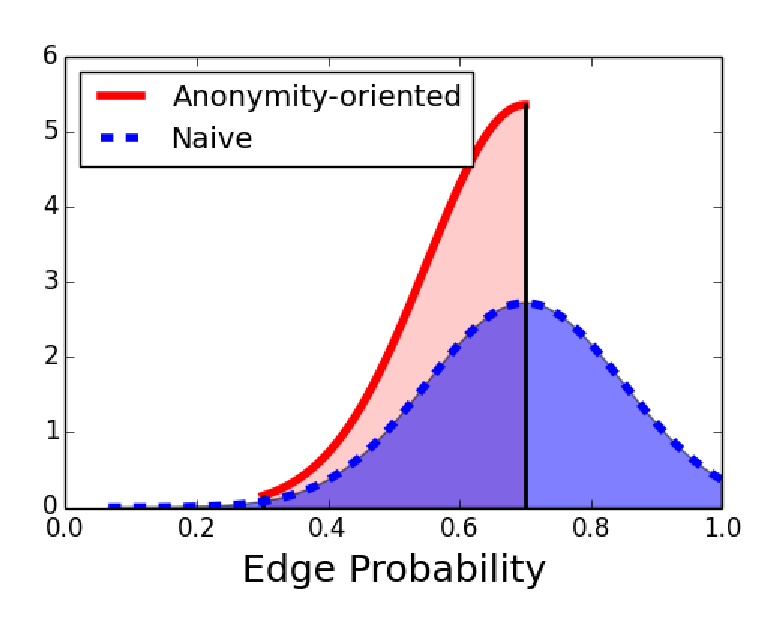
\includegraphics[width=1\textwidth]{ill/anonymityEP.eps}
    \end{minipage}
  }
  \subfigure[]{\label{fig:constraintRelax}  %(22)
    \begin{minipage}[l]{0.45\columnwidth}
      \centering
      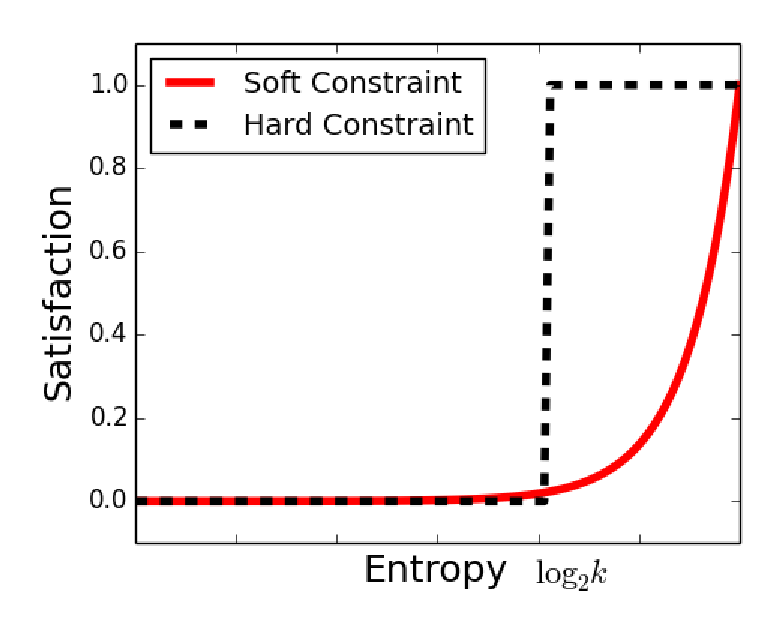
\includegraphics[width=1\textwidth]{ill/constraint.eps}
    \end{minipage}
  }
    \vspace{-0.7em}
    \caption{(a) Anonymity-oriented edge perturbing; (b) Relaxing $k$-obfuscation constraint.}
    \vspace{-1.5em}
\end{figure}






\subsubsection{Proof Sketching the Heuristic}
\label{sec:prooooof}
% {\todo{I still think this section is too detailed and no one will read such theorems and proofs, especially near the end of the paper. If that is not the formal proof, then the formal proof is what?? I would suggest describing the rational only here possibly with some figure and example...}}

We proceed to elaborate the rationality this anonymity-oriented edge perturbing scheme briefly. The formal detail proof of our heuristic is available in tech report. The core idea is to maximize the entropy of degree uncertainty matrix (referred to as ME). 

To facilitate further discussion, we consider the extreme case $k$-obf, which poses a set of hard constraints over the anonymized solution. Let the constraint being $k$-obf be $\mathbb{C}$, $k-$obfuscate a vertex $v$ be $\mathtt{c}_{v}$. 
According to Definition~\ref{def:obf}, $k-$obf can be expressed as joint satisfaction of $\lbrace c_{v}~:~v \in V \rbrace$ since the uncertain graph is said to be $k$-obf iff it $k-$obfuscates all the vertices. The formal definition as follows. 
\begin{equation}
    \mathbb{C}= \prod_{v \in V} \mathtt{c}_{v}
\end{equation}
where
\begin{equation*}
        \mathtt{c}_{v}:=
        \begin{cases}
                1  & H(Y_{P(v)}) \geq \log_{2}{k} \\
                0  & otherwise \\
         \end{cases}
\end{equation*}
In other words, given an uncertain graph, its satisfaction evaluation of $\mathbb{C}$ indicates whether it achieves the desirable anonymity level ($k$-obf).

However, as shown in Figure~\ref{fig:constraintRelax}, a single constraint at the vertex level is either fully satisfied or fully violated. It limits the optimization opportunity of methods based on local search. In this work, we model the individual constraint $c_{v}$ to a fuzzy relation in which the satisfaction of a constraint is a continuous function of its variables' values 
% ({\ie}, edge probabilities),  wrong statement 
({\ie}, the entropy $H(Y_{P(v)}$),
going from fully satisfied to fully violated as follows. 
\begin{equation}
    C_{v} = e^{H(Y_{P(v)})-\log_{2}{|V|}}
    \label{eq:approximate}
\end{equation}

\begin{theorem}
Let $\Omega$ presents the domain of degree values in the original uncertain graph, the maximization of the provided anonymity $\mathbb{C}$ is equivalent to the maximization of the following function:
  \begin{equation}
      \sum_{\omega \in \Omega} s(\omega) \cdot H(Y_{\omega}) 
      \label{eq:anonymity}
  \end{equation} 
\end{theorem}

{\bf Proof Sketch:} First we can see that 
\begin{align*}
    \mathcal{C} &= \prod_{v \in V} \mathtt{c}_{v} 
                 = \prod_{\omega \in \Omega} \underbrace{\mathtt{c_{\omega}} \ldots \mathtt{c}_{\omega}}_{s(\omega)} 
\end{align*}
Taking logarithm for both sides and combining with the approximation equation~\ref{eq:approximate}, we can see that 
\begin{align*}
    \log(\mathcal{C}) &=\sum_{\omega \in \Omega} s(\omega) \log(\mathtt{c_{\omega}}) \\
                      &=\sum_{\omega \in \Omega} s(\omega) \big[ H(Y_{\omega})-\log_{2}{|V|} \big] \\
                      &=\sum_{\omega  \in \Omega} s(\omega) H(Y_{\omega}) -\sum_{\omega  \in \Omega} \log_{2}{|V|}
\end{align*}
Therefore, after removing the constant $\sum_{\omega} \log_{2}|V|$ from $\log(\mathcal{C})$, our goal is actually to maximize Equation~\ref{eq:anonymity}. It provides us with the relation between the global anonymity and the level of disorder of the degree uncertainty matrix.  

% option a: use lemma with number, cross reference can be graceful 
\begin{theorem}
The maximization of Equation~\ref{eq:anonymity} is equivalent to maximization of the following function:
  \begin{equation}
      \sum_{\omega \in \Omega} s(\omega) \cdot H(Y_{\omega}) =\big[ \sum_{v \in V} H(d_{v})\big] + |V|\log{|V|}-|V|H(\Omega)
  \end{equation}
The equation stems from the coding length of degree uncertainty matrix from different perspectives (row and column).\footnote{More detail of it is available in tech report.}
\end{theorem}
It provides us with the mechanism for gaining better anonymity, namely increasing the degree uncertainty per vertex $H(d_{v})$. 

\begin{theorem}
As implied by the Central Limit Theorem, $d_{v}$ may be approximated by the normal distribution $\mathcal{N}(\mu,\sigma^2)$, where $\mu=\sum_{e \in \mathcal{E}^{v}} p(e)$ and $\sigma^2=\sum_{e \in \mathcal{E}^{v}} p(e)-p(e)^2$. Therefore, its entropy may be approximated by the differential entropy of the normal distribution $\frac{1}{2} \ln(2\pi\sigma^2) + \frac{1}{2}$. For a given $p(e)$, its gradient ascent is proportion to $1-2\cdot p(e)$. 
\end{theorem}
Targeting at high entropy, we apply the gradient ascent method---$\hat{p}(e)=p(e)+ \big( 1-2\cdot p(e) \big) \cdot r_{e} $ for achieving the increase of degree entropy and the anonymity gain.


